\documentclass[letter,answers,addpoints]{exam}
\usepackage{algpseudocode}
\usepackage{listings}
\usepackage{tabularx}
 \usepackage{graphicx}

\usepackage{DejaVuSansMono}
%\renewcommand*\familydefault{\ttdefault} %% Only if the base font of the document is to be typewriter style
%\usepackage[T1]{fontenc}

\pagestyle{headandfoot}
\runningheadrule
\header{CIS 2168}{Basic Algorithm Analysis}{}
\lfoot{}
\cfoot{Page \thepage\ of \numpages}
\rfoot{\makebox[1in]{\hrulefill}
	\pointsonpage{\thepage} points}




\begin{document}
	\lstset{language=Java, basicstyle= \ttfamily\small,  showstringspaces=false} 
	\vspace*{0.15in}
	\makebox[4in]{Name:\enspace\hrulefill}
	\vspace{0.25in}
	
	
	Here are some basic rules for calculating the Big O for some $T(n)$ or an algorithm.
	
	\begin{enumerate}
		\item Only the highest degree of $ n $ matters.  For example $$ T(n) =n^3 +5n^2 +10^7  \rightarrow O(n^3) $$ since once $ n $ becomes super-massively huge,  the other terms just stop mattering.
		\item Constant factors don't matter. $ T(n)  = 500n$ and  $ T(n)  = 0.005n$ both $O(n)$. Again, as $ n $ becomes bigger, these constants stop mattering; what matters is the rate of growth. Example: $$T(n) = 50n^3 - 2n^2 +400 \rightarrow O(n^3)$$
		\item  Counting the number of nested loops usually works.
	\end{enumerate}

	Demo this assignment to the Professor or TA.
	\newpage
	
	\begin{questions}
		
		
		
		
		\uplevel{For each of the following $T(n)$, write the corresponding Big O time complexity.  Some series may require research.}
		
		\question[2]  $T(n)= n^2 +3n +2$	\answerline[$ O(n^2) $]
		\question[2]  $T(n)= (n^2 + n)(n^2 + \frac{\pi}{2}) $	\answerline[$ O(n^4) $]
		\question[2]  $T(n)= 1 + 2 + 3 + \dots + n-1 + n$	\answerline[$ O(n^2) $]
		\question[2]  $T(n)= 1^{2} + 2^{2} + 3^{2} + \dots + (n-1)^{2} + n^{2}$	\answerline[$ O(n^3) $]
		\question[2]  $T(n)= 10$	\answerline[$ O(1) $]
		\question[2]  $T(n)= 10^{100}$	\answerline[$ O(1) $]
		\question[2]  $T(n)= n + \log n$	\answerline[$ O(n) $]
		\question[2]  $T(n)= 12\log(n) + \frac{n}{2} - 400$	\answerline[$ O(n) $]
		\question[2]  $T(n)= (n+1)\cdot\log(n) - n $	\answerline[$ O(n\log(n)) $]
		\question[2]  $T(n)= \frac{n^4 +3n^2 +2n}{n}$	\answerline[$ O(n^4) $]
		
		
		\newpage 

	
		\question[4] What is the time complexity to  get an item from a specific index in an ArrayList?
		\begin{solution}[\stretch{1}]
			$ O(1) $ on average	
		\end{solution}


		\question[3] What is the time complexity remove an item in the middle of an ArrayList?
		\begin{solution}[\stretch{1}]
			$ O(n) $
		\end{solution}
		
		\question[3] Why?
		\begin{solution}[\stretch{1}]
		Because we shift half the items in the list.
		\end{solution}
		
		
		
		\question[3] What is the \textbf{average} time complexity to add an item to the end of an ArrayList?
		\begin{solution}[\stretch{1}]
		$ O(1) $ on average	
		\end{solution}
		
		
		\question[3] What is the \textbf{worst case} time complexity to add an item to the end of an ArrayList?  What if you have to or don't have to reallocate?
		
		\begin{solution}[\stretch{1}]
		$ O(n) $	
		\end{solution}
		
		\question[4] Taking this all into account, what situations would an ArrayList be the appropriate data structure for storing your data?
		\begin{solution}[\stretch{1}]
		When we are doing a lot of adding to the end of the arraylist	 and doing lots of get or set operations.   Other explanations are acceptable.
		\end{solution}
		
\newpage

% TODO: \usepackage{graphicx} required
\begin{figure}[h!]
	\centering
	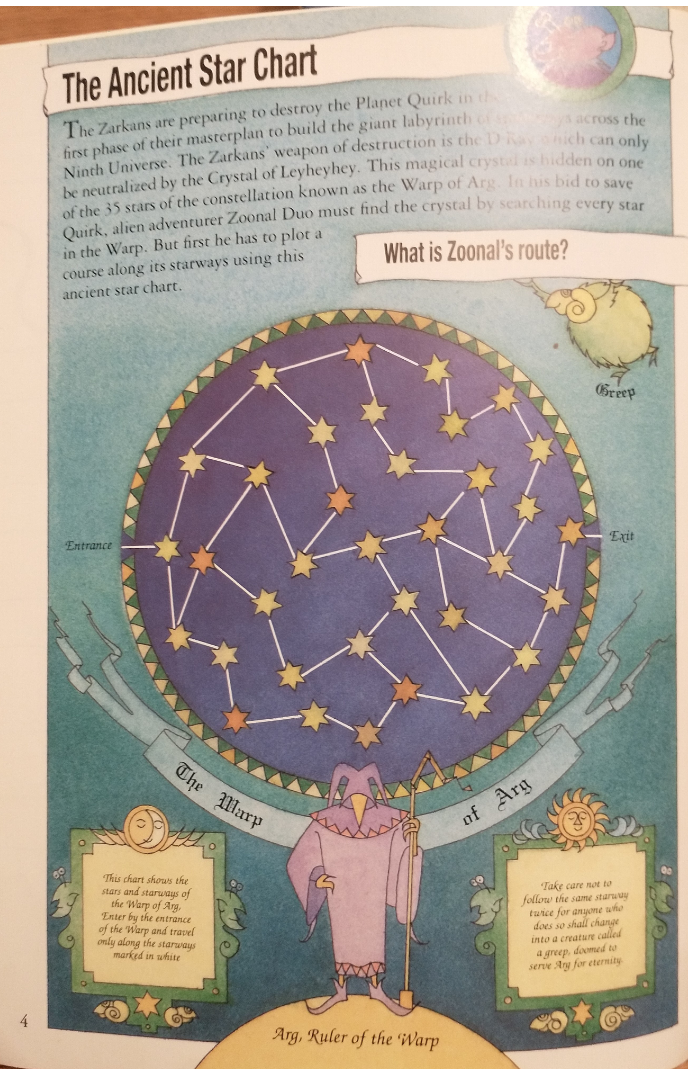
\includegraphics[width=0.7\linewidth]{starchart}
	\caption[Please look at the above puzzle, taken from Sarah Dixon’s \textit{Map \& Maze Puzzles} and answer the questions on the next page.]{Please look at the above puzzle, taken from Sarah Dixon's \textit{Map \& Maze Puzzles }and answer the questions on the next page.}
	\label{fig:starchart}
\end{figure}

\newpage
	
\question[10] 
The attached puzzle, while from a children’s puzzle book, is actually a very interesting graph
theory problem, known as the Rudrata Path or Hamiltonian Path. What is the Rudrata Path problem
and how does it correspond to the above puzzle?

\begin{solution}[\stretch{1}]
Zoonal's route requires not visiting the same starway (edge) twice but requires him to visit every star.

Having to visit every star (vertex) makes this problem equivalent to finding a Rudrata Path.
\end{solution}

\question[10] Suppose we generalized the above puzzle so that there was any number of stars, rather than
just 35. Let the number of stars in the above puzzle be defined as $n$. If there are $n$ stars and there are starways between any number of random pairs of stars such that a solution exists, how many paths would an algorithm need to check in order to check to find the solution?



\begin{solution}[\stretch{1}]
	Expected answer is $O(n!)$ as there are that many paths to check in brute force.
	
	
	Info for TA's: problem is NP complete.
	
\end{solution}

	\newpage
	\uplevel{\texttt{bogosort} attempts to sort a list by shuffling the items in the list.  If the list is unsorted after shuffling, we continue shuffling the list and checking until it is finally sorted.}
		\question[5] What is the worst case run time for \texttt{bogosort}?
		\begin{solution}[\stretch{1}]
			Student can answer Infinite or indeterminate.
		\end{solution}
		
		\question[5] Why?
		\begin{solution}[\stretch{1}]
			Student can answer it either goes on forever as there's no guarantee to end or that it runs through all possible permutations of list.
		\end{solution}
		
		\question[5] What is the average case run time for \texttt{bogosort} (Hint: think about a deck of cards )? 
		\begin{solution}[\stretch{1}]
		$ O((n+1)!) $ or $ O(n \cdot n!) $, as the latter reduces to the former.
			
			
		\end{solution}
		
		\question[5] Why?
		
		\begin{solution}[\stretch{1}]
			We run through all possible permutations and find a sorted one approximately half way through.
		\end{solution}
		
	\newpage
	\question[20]  For each of the methods you wrote in Lab 2, figure out the time complexity of the method you wrote.
	To turn in this portion, attach a printout of the code and specify the time complexity of each.
	
	
		
	\end{questions}
	
\end{document}
